% !TEX TS-program = xeLaTeX

\documentclass[]{beamer}
\usepackage{standalone}
\usepackage{graphicx}
\graphicspath{{../figs/}}

\usepackage{ amssymb }
\usepackage{amsmath}
\usepackage{rotating}
\usepackage{fontspec}
\usepackage{microtype}


%%%%%%%%%%%%%%%%%%%%%%%%%%
% PGFPLOTS
\usepackage{pgfplots}
\pgfplotsset{compat=1.12}
\usepackage{booktabs, array} % Generates table from .csv
\usepackage{pgfplotstable}

\newcolumntype{C}[1]{>{\centering\arraybackslash}m{#1}}

\pgfplotstableset{percent style/.style=}
		}},
		%
		%
		every head row/.style={after row=\midrule},
	}
	
%%%%%%%%%%%%%%%%%%%


\usepackage{arrayjobx}
\usepackage{xifthen}
\usepackage{tikz,textcomp}
\usetikzlibrary{positioning}
\newcommand{\fullpagetikz}[1]{{\input{#1}}}
\newcommand{\widthtikz}[2]{\resizebox{#1\textwidth}{!}{\input{#2}}}
\newcommand{\fullwidthtikz}[1]{\resizebox{0.9\textwidth}{!}{\input{#1}}}

%%%%%%%%%%%%%Bibliography
\usepackage[backend=bibtex, url=false,
bibstyle=ieee,firstinits=true]{biblatex}
\bibliography{master.bib}
\renewcommand*{\thefootnote}{} %No symbol or marker
\renewcommand{\footnotesize}{\scriptsize}
%%%%%%%%%%%%%%%%%


\usepackage{xcolor}
\definecolor{chamois}{RGB}{255,255,240}
\definecolor{darkbrown}{RGB}{124,79,0}
\definecolor{UniBlue}{RGB}{83,101,130}

\definecolor{hellgelb}{rgb}{1,1,0.8}
\definecolor{colKeys}{rgb}{0,0,1}
\definecolor{colIdentifier}{rgb}{0,0,0}
\definecolor{colComments}{rgb}{1,0,0}
\definecolor{colString}{rgb}{0,0.5,0}


\usefonttheme{professionalfonts} 

\newcommand{\topline}{%
  \tikz[remember picture,overlay] {%
    \draw[brown,ultra thick] ([yshift=-1.6cm]current page.north west)-- ([yshift=-1.6cm,xshift=\paperwidth]current page.north west);} }

\renewcommand{\topline}{}

\setbeamertemplate{frametitle}{\begin{minipage}[b][1.6cm][c]{\textwidth}%
	\centering%
	\insertframetitle\\\insertframesubtitle
	\end{minipage}}
	

\addtobeamertemplate{frametitle}{}{\topline%
}

\setbeamertemplate{navigation symbols}{}
\setbeamercolor{background canvas}{bg=chamois}
\setbeamercolor{itemize item}{fg=brown}
%\setbeamertemplate{itemize item}{\maltese}
\setbeamercolor{itemize subitem}{fg=brown}
%\setbeamertemplate{itemize subitem}{\begin{rotate}{90}$\diamondsuit$\end{rotate}}

\setbeamercolor{title}{fg=UniBlue}
\setbeamercolor{frametitle}{fg=UniBlue}
\setbeamercolor{structure}{fg=UniBlue}

\setbeamercolor{author}{fg=darkbrown}
\setbeamercolor{institute}{fg=darkbrown}
\setbeamercolor{date}{fg=darkbrown}

\setbeamercolor{block title}{bg=darkbrown!40,fg=darkbrown!90}
\setbeamercolor{block body}{bg=darkbrown!20,fg=UniBlue}

\setbeamercolor{math text}{fg=darkbrown}
\setbeamercolor{math text displayed}{fg=darkbrown}
\addtobeamertemplate{block begin}{%
  \setlength{\textwidth}{0.8\textwidth}%
}{}

\setbeamercolor{block title alerted}{bg=yellow!60,fg=red}
\setbeamercolor{block body alerted}{bg=hellgelb!80,fg=UniBlue}


%%%%%%%%%%%%%%%%%%%%%%%%%%%%%%%%%%%%%%%%%%%%%%%%%%%%%%%%%%%%%%%%%%%%%%%%%%%%%%%%%%%%%%%%%%
\renewcommand{\c}{\tilde{c}}
\newcommand{\s}{\tilde{s}}
\newcommand{\x}{\tilde{x}}
\renewcommand{\t}{\tilde{t}}
\newcommand{\N}{\mathbb{N}}
\newcommand{\R}{\mathbb{R}}
\newcommand{\V}{\mathcal{V}}
\renewcommand{\B}{\mathcal{B}}


\author{Lyndon White}
\institute{School of EE\&C Engineering\\The University of Western Australia}
\title{Generating Sentences from the Sum of their Contents}
\subtitle{A greedy algorithms for sentence generation from sum of word embeddings representations}

\begin{document}
\centering %Center everywhere
\frame{\maketitle}

\begin{frame}{We have turned sentences into numeric vectors, now we want to turn them back.}

	\begin{enumerate}
		\item<1-> It was the best of times, it was the worst of times
		\item<1->  $[−0.79, 1.27, 0.28, ..., −1.29]$
		\item<1-> It was the worse of times, it was the best of times
	\end{enumerate}
\end{frame}

\begin{frame}{We have turned sentences into numeric vectors, now we want to turn them back.}
	Input Sentences \hfill Manipulate Numbers \hfill Output Sentences
	\vspace{0.5cm}
	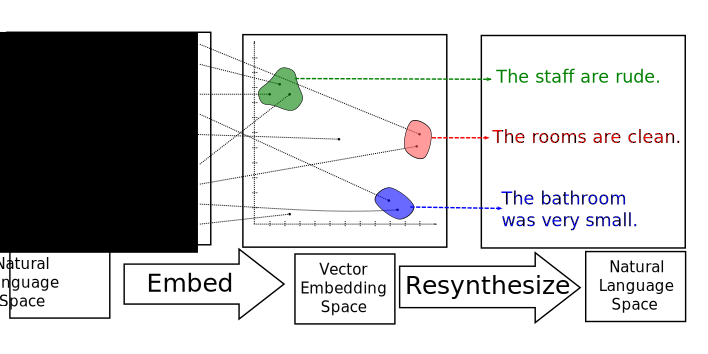
\includegraphics[scale=0.5]{workflow}
\end{frame}

\begin{frame}[label=twostep]{We can break the problem down into two subproblems.}
	\vfill

	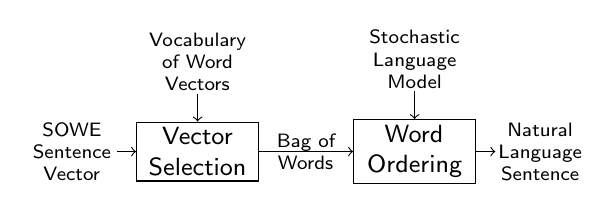
\begin{tikzpicture}[
		every node/.style={ text width=4em,
			align=center,
			font=\scriptsize\sffamily,
			inner sep=1pt
		},
		proc/.style= {draw,
			font=\small\sffamily,
			inner sep = 2pt
		}
		]
		\onslide<1,3->{
			\node (input) [inner sep=-4pt] {SOWE Sentence Vector};
			\node (selection) [proc, right = 0.7em of input]{Vector\\ Selection};
			\node (vocab) [above = 1em of selection]{Vocabulary of Word Vectors};
			\draw[->] (input) -- (selection);
			\draw[->] (vocab) -- (selection);
		}
		\onslide<2->{
			\node (ordering) [proc, right = 3.4em of selection]{Word\\ Ordering};
		}

		
		\draw[->] (selection) -- (ordering) node[midway] {Bag of Words};
		\onslide<2,3->{
			\node (output) [inner sep=-4pt, right=0.7em of ordering] {Natural Language Sentence};
			\node (lm) [above = 1em of ordering] {Stochastic Language Model};
			\draw[->] (lm) -- (ordering);
			\draw[->] (ordering) -- (output);
			
		}
	\end{tikzpicture}
	\vfill
	\only<1>{Vector Selection: Select which word vectors go into the sum}
	\only<2>{Word Ordering: Find them most likely order of words}
	\only<3>{They are however both NP-Hard
		%\\But both are similar to well studied problems
		}
	\vfill
\end{frame}

\newcommand{\vectorselectionproblemdefn}{Find the inclusion vector $\c=[c_1,c_2,...c_n]\in\N_0^n$ that for $\displaystyle f(\c) = \sum_{\x_j\in\V}\:\x_{j}\,c_{j}$ we have $\min d(\s,f(\c))$}

\begin{frame}{We solve the objective function to get a bag of words.}
	\vectorselectionproblemdefn
	\vfill
	\begin{description}
		%\item<1->[Target Output] It was the best of times, it was the worst of times
		\item<2->[Input Vector]  $\s=[−0.79, 1.27, 0.28, ..., −1.29]$
		\vfill
		\item<3->[Vector Selection] $\displaystyle
			\begin{aligned}%
			f(\c)&=\quad1\times[−0.19, 0.50, 0.14, ..., −0.59]\\
			&\quad+2\times[-0.15, 0.19, 0.03, ..., -0.17]\\
			&\quad+\qquad...\\
			&\quad+0\times[−0.19, 2.10, 1.34, ..., 1.20]\\
			&\quad+1\times[−0.79, 1.27, 0.28, ..., −1.29]
		\end{aligned}
		$
		\vfill
		\item<4->[BOW] \texttt{\{best: 1,times: 2, worst: 1, \\it: 2, of: 2, the: 2, was: 2,, : 1\}}
	\end{description}
\end{frame}

\begin{frame}{How to solve objective function? Greedily}
	\vectorselectionproblemdefn
		\vfill
	\begin{itemize}
		\item<1-> Similarities to Knapsack family of problems.
		\item<2-> Very high dimensionality of selection vector\begin{itemize}
			\item $n$ is given by vocabulary size ($n=|\V|$)
			\item $\approx40,000$ for Brown Corpus\hfill $\approx170,000$ for Books Corpus\hspace{1em}
			\end{itemize}
		\item<3-> A Greedy Algorithm is linear time in $n$ 
	\end{itemize}
	\vfill
\end{frame}

\newcommand{\vectorselectionproblemdefnalt}{Find the bag of vectors $\B$ (a multi-subset of $\V$), such that $\displaystyle \Sigma(\B)=\sum_{\x_a\in\B}\x_a$ we have  $\min d(\s,\Sigma(\B))$}

\begin{frame}{Alternative notation for vector selection problem}
	Rather than writing:\\
		\vectorselectionproblemdefn
	\vfill
	Write:\\
		\vectorselectionproblemdefnalt
	\vfill
	
\end{frame}


\begin{frame}{Greedy Addition: where you add the best vector to your current bag, and repeat.}
	\vectorselectionproblemdefnalt
	\vfill
	\begin{enumerate}
		\item For each vector $\x_j$ in the vocabulary consider  $d(\s, \Sigma(\B)+\x_j)$
		\item Add the vector that gets closest the bag. $\B\leftarrow\B\cup\{\x_\star\}$
			\begin{itemize}
				\item unless adding nothing would be better -- then terminate
			\end{itemize}
		\item Repeat
	\end{enumerate}
	\vfill
\end{frame}

\begin{frame}{A 1 dimentional example of greedy additon}
	\vectorselectionproblemdefnalt
	\vfill
	Consider $\V=\{24,25,100\}$ \hfill $\s=148$ \hfill $d(x,y)=|x-y|$
	\begin{enumerate}
		\item<1-> $\B=[]$ \hfill $d(\s,\Sigma(\B))=|148-0|=149$ 
		\item<2-> $\B=[100]$ \hfill $d(\s,\Sigma(\B))=|148-100|=48$ 
		\item<3-> $\B=[100,25]$ \hfill $d(\s,\Sigma(\B))=|148-(100+25)|=23$ 
		\item<4-> $\B=[100,25,24]$ \hfill $d(\s,\Sigma(\B))=|148-(100+25+24)|=1$ 
		\item<5-> $\B=[100,25,24]$ \hfill No improvement possible \hfill $d(\s,\Sigma(\B))=1$ 
	\end{enumerate}
	\vfill
	\onslide<5->{Fell for greedy trap}
	\vfill
	\note{If we knew the other elements of hte bag would be 100, and 24 then we would not have put in a 25}
\end{frame}

\begin{frame}{1-Subsitution: Lessen the greed by reconsidering past choices}
	\vectorselectionproblemdefnalt
	\vfill
	\begin{enumerate}
		\item Consider each word vector in the current bag $\x_a\in\B$
		\item Would deleting it improve the score? $d(\s,\Sigma(\B)-\x_a)<d(\s,\Sigma(\B))$ ?
		\item Can it be swapped for another word to improve the score?
		$\exists \x_b\in\V$ such that
		$d(\s,\Sigma(\B)-\x_a+\x_b))<d(\s,\Sigma(\B))$ ?
	\end{enumerate}
\end{frame}

\begin{frame}{A 1 dimentional example of 1-substitution}
	\vectorselectionproblemdefnalt
	\vfill
	Consider $\V=\{24,25,100\}$ \hfill $\s=148$ \hfill $d(x,y)=|x-y|$
	\begin{enumerate}
		\item<1-> $\B=[100,25,24]$ \hfill $d(\s,\Sigma(\B))=|148-(100+25+24)|=1$ 
		\item<2-> $\B=[100,24,24]$ \hfill $d(\s,\Sigma(\B))=|148-(100+24+24)|=0$ 
		\item<3-> $\B=[100,24,24]$ \hfill Perfect\hfill $d(\s,\Sigma(\B))=0$ 
	\end{enumerate}
	\vfill
	\onslide<3->{Fixed, but there are deeper greed traps, that can be constructed.}
	\vfill
\end{frame}


\begin{frame}{Run until converance}
	\vfill
	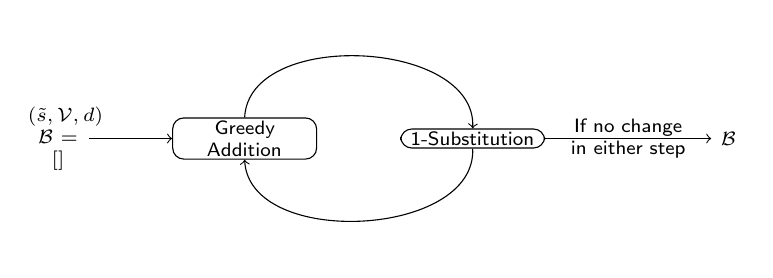
\begin{tikzpicture}[
		every node/.style={ text width=5em,
			align=center,
			font=\scriptsize\sffamily,
			inner sep=1pt,
		},
		]

		\node (input) [text width=2em] {$(\s,\V,d)$\\$\B=[]$};
		\node (addition) [draw, rounded corners, right = 3em of input]{Greedy Addition};
		\node (substitution) [draw, rounded corners, right = 3em of addition]{1-Substitution};
		\node (output) [right = 6em of substitution,text width=1em] {$\B$};
		\draw[->] (input) -- (addition);
		\path[->] (addition) edge [bend left=90,looseness=1] (substitution);
		\path[->] (substitution) edge [bend left=90,looseness=1] (addition);
		\draw[->] (substitution) -- (output) node[midway] {If no change in either step};
			
	\end{tikzpicture}
		\vfill
\end{frame}

\begin{frame}{Experimental Setup: Preprocess corpora to only use known words.}
	\begin{itemize}
		\item<1-> For word embeddings, we use pretrained GloVe \footfullcite{pennington2014glove}
		\item<2-> Restrict Vector vocab to only words used in corpora
		\item<2-> Preprocess Corpora to remove sentences with words not found in vocabulary.
	\end{itemize}
\end{frame}

\begin{frame}{Experimental Setup: we used the Brown, and the Books Corpus}
	\footfullcite{francis1979brown}
	\footfullcite{moviebook}
				
	\begin{columns}[T]
		\begin{column}{0.5\textwidth}
			\textbf{Brown}
			\begin{itemize}
				\item 40,485 unique words
				\item 42,004 sentences
				\item Sentence Length Q3: \\\hfill 25 words
				\item Extracts from 500 varied works from 1961
			\end{itemize} 
		\end{column}
		\begin{column}{0.5\textwidth}
			\pause
			\textbf{Books}
			\begin{itemize}
				\item 178,694 unique words
				\item 66,464 sentences 
				\item Sentence Length Q3: \\\hfill 17 words
				\item 11,038 unpublished novels, we use just a small random subset
			\end{itemize}
		\end{column}
	\end{columns}

\end{frame}

\begin{frame}{Results: The more dimentions used in the word performance, the better the recovery.}
	\begin{table}
		\pgfplotstabletypeset[col sep=comma,fixed zerofill, precision=3,column type=C{3em},
		columns/Corpus/.style={string type},
		columns/Word Embedding Dimensions/.style={string type},
		columns/Portion Perfect/.style={percent style, precision=1},
		every head row/.style={
			after row=\midrule
		}]{../data/selection_overall_len_scores.csv}
	\end{table}
\end{frame}


\begin{frame}{}
	\only<1>{\frametitle{Result: The longer the sentence, the worse recovery}}
	\only<2>{\frametitle{Result: The larger the vocabulary, the worse recovery}\topline}
	
	\pgfplotstableread[col sep=comma,header=has colnames]{../data/selection_len_scores.csv}{\sellenscores}
	
	\begin{tikzpicture}
	\begin{axis}[xlabel=Ground Truth Sentence Length,
	ylabel=Mean Jaccard Index,
	width=0.9\textwidth,height=0.5\textwidth,cycle list name=exotic]
	\addplot table [y=brown_glove50_jaccard_mean,x=ground_len]{\sellenscores};
	\addplot table [y=brown_glove100_jaccard_mean,x=ground_len]{\sellenscores};
	\addplot table [y=brown_glove200_jaccard_mean,x=ground_len]{\sellenscores};
	\addplot table [y=brown_glove300_jaccard_mean,x=ground_len]{\sellenscores};%
	\addplot table [y=books_0_01_glove300_jaccard_mean,x=ground_len]{\sellenscores};
	\legend{50D Brown, 100D Brown, 200D Brown,300D Brown, 300D Books}					
	\end{axis}
	\end{tikzpicture}	
\end{frame}

\againframe<1>{twostep}
\againframe<3>{twostep}
\againframe<2>{twostep}

\begin{frame}{Now that we have a bag of words, we need to order them to get a sentence.}
	\vfill
		Find the most-likely ordering, of the bag of words.
	\vfill
	\begin{description}
		\item<1->[Input Vector]  $[−0.79, 1.27, 0.28, ..., −1.29]$
		\item<1->[Bag of Words]  \texttt{\{best: 1,times: 2, worst: 1,\\ it: 2, of: 2, the: 2, was: 2,, : 1\}}
		\vspace{1em}
		\item<1->[Output Sentence] It was the worse of times, it was the best of times
	\end{description}
	\vfill
\end{frame}

\begin{frame}{A language model tells us the probability of a word sequence.}
	\begin{itemize}
		\item based on corpus statistics
		\item Trigram language model: $P(W_3=buns\:|\:W_1=hot, W_2=crossed)$
		\item Note the Markov Assumption
		\pause
		\item Bayesian Chain Rule: probability of sequence \\$P([w_1,w_2,w_3,w_4,w_5])=$
		$$\qquad \quad P(w_1,w_2)\cdot P(w_3|w_1,w_2)\cdot P(w_4|w_2,w_3) \cdot P(w_5|w_3,w_2)$$
		
	\end{itemize}
	
\end{frame}

\begin{frame}<1>{Word Sequencing as a Travelling Salesman Problem}
	\widthtikz{0.5}{../figs/ordergraph.pgf}
	\begin{itemize}
		\item an edge $(w_aw_b)\to (w_bw_c)$ has cost $=-\log(P(w_c\:|\:w_aw_b)$
		\item Variation on Generalised Asymmetric Travelling Salesman (GA-TSP)
	\end{itemize}
	\footfullcite{Horvat2014}
\end{frame}

\begin{frame}{A graph representation of word sequencing problem}
	\fullwidthtikz{../figs/ordergraph.pgf}
\end{frame}

\begin{frame}{The problem is defined with certain constrains.}
	\widthtikz{0.5}{../figs/ordergraph.pgf}
	\begin{description}
		\item<1-> [Single Path] from $\blacktriangleright\triangleright$ to $\triangleleft\blacktriangleleft$
		\begin{itemize}
			\item every word node entered must be exited
			\item no subtours
		\end{itemize}
		\item<2-> [Districts] Every word must be used exactly once
		\item<3-> [Markov Consistency] $(w_aw_b)\to (w_cw_d) \iff w_b==w_c$
	\end{description}
\end{frame}



\begin{frame}{TSP can be solved with MIPs}
	\begin{itemize}
		\item After rewriting word ordering as a TSP:
		\item Rewrite it as a Mixed Integer Programming (MIP) Problem
		\item There exist very fast MIP solvers.
		\item This gave multiple orders of magnitude improvement over Best First Search.
	\end{itemize}
\end{frame}

\begin{frame}{Experimental Setup: Language Modeling}
	\begin{itemize}
		\item<1-> Preliminary Investigation on 10\% of the books corpus used in previous investigation ~6000 sentences.
		\item<1-> Further subset to length 18 or less
		\vfill
		\item<2-> Language model trained on ~6 million sentences.
		\item<2-> Use Kneser Ney Smoothing. \footfullcite{kneser1995improved}
		
	\end{itemize}
\end{frame}

\begin{frame}{Results: This seems to work alright, for short sentences.}
	\begin{table}
		\pgfplotstabletypeset[col sep=comma, fixed zerofill, precision=3,column type=C{3em},
		columns/Input/.style={string type},
		columns/Portion Perfect/.style={percent style, precision=1},
		columns/Portion Perfect (Feasible only)/.style={percent style, precision=1},
		columns/Feasible/.style={percent style, precision=1},
		every head row/.style={
			after row=\midrule
		}]{../data/prelim_ordering.csv}
	\end{table}
	\vfill
	Prelim results on 6000 examples from Books Corpus. Length 18 or less.
	\vfill
\end{frame}



\pgfplotstableread[col sep=comma,header=has colnames]{../data/prelim_ordering_len_scores.csv}{\ordlenscores}
\pgfplotstableread[col sep=comma,header=has colnames]{../data/prelim_ordering_len_scores_oracle.csv}{\ordlenscoresoracle}

\begin{frame}{Result: The longer the sentence, the worse recovery of order.}

	\begin{tikzpicture}
	\begin{axis}[xlabel=Ground Truth Sentence Length,
	ylabel=Portion Exactly Matched,
	width=0.9\textwidth,height=0.5\textwidth,cycle list name=exotic]
	\addplot table [y=Exact_Matches,x=ground_length]{\ordlenscores};
	\addplot table [y=Exact_Matches,x=ground_length]{\ordlenscoresoracle};
	\legend{Generated BOWS, Oracle BOWS}
	\end{axis}
	\end{tikzpicture}	
\end{frame}

\begin{frame}{The overall performance is tolerable, particularly for short sentences}
	\begin{itemize}
		\item 0.75 BLEU is very good, 62\% perfect recreation is usable.
		\item This does come from most sentences being short though.
		\item This is the first work to present quantitative results for sentence generation based on any sentence vector representation.
		
	\end{itemize}
\end{frame}

\begin{frame}{As expected, expodential time taken for ordering}
	\begin{tikzpicture}
	\begin{axis}[xlabel=Ground Truth Sentence Length,
	ylabel=Time Taken (s),
	width=0.9\textwidth,height=0.5\textwidth,cycle list name=exotic]
	\addplot table [y=Time_taken,x=ground_length]{\ordlenscores};
	\addplot table [y=Time_taken,x=ground_length]{\ordlenscoresoracle};
	%\legend{Generated BOWS, Oracle BOWS}
	\end{axis}
	\end{tikzpicture}	
\end{frame}

\againframe<2>{twostep}
\againframe<3>{twostep}



\begin{frame}{Conclusion: Split the sentence generation into selection then ordering.}
	\begin{itemize}
		\item<1->Selection: Greedy Method
		\begin{itemize}
			\item Broad generalisation of Knapsack Problem
			\item Input: vector
			\item Greedy Addition + 1-Substitution til converge
			\item Output: BOW
		\end{itemize}
		\vfill
		\item<2->Ordering: most likely order over log-likelyhoods 3grams.
		\begin{itemize}
			\item Variation of Traveling Salesman
			\item Input: BOW
			\item Rewrite as GA-TSP, then as MIP
			\item Output: Most likely order of words
		\end{itemize}
	\end{itemize}
\end{frame}




\end{document}